\documentclass[10pt]{article}
%-*-*-*-*-*-*-*-*-*-*-*-*-*-*-*-*-*-*-*Packages--*--*--*--*--*--*--*--*--*--*--*--*--*

\usepackage[usenames,dvipsnames]{pstricks}
\usepackage{epsfig}
\usepackage{pst-grad} % For gradients
\usepackage{pst-plot} % For axes

\usepackage{amsmath}
\usepackage{tikz}
\usepackage{epigraph}
\usepackage{lipsum}
\usepackage{mdframed}
\usepackage{fancyhdr}
 \usepackage[utf8]{inputenc}
\usepackage{hyperref} 
\usepackage[spanish]{babel}
%\usepackage{simpsons}
%\usepackage[dvips]{graphicx}
\usepackage{amsmath}
\usepackage{amsthm}
%\usepackage{textcomp}
\usepackage{amssymb}
\usepackage{latexsym}
\usepackage{graphicx}
%\usepackage[ansinew]{inputenc}
\usepackage{color}
%\usepackage{pstricks, pst-node, pst-plot, pst-circ}
%\usepackage{moredefs}
%\usepackage{pstricks}
%\usepackage{pst-circ}
%\usepackege{pst-node}
%\usepackage{pst-plot}
\usepackage{moredefs}
%\usepackage{mcode}
%\usepackage[above]{placeins}
\usepackage{fancybox}
\usepackage{subfig}
\usepackage{float}
%\usepackage{mcode} para colorear codigo de matlab
\usepackage{xcolor}
\usepackage{wallpaper}
\usepackage{textcomp}

\oddsidemargin -0.2in \textwidth 7.0in \topmargin -0.9in \textheight
9.0in
\parindent 3em
\hyphenation{e-jem-plo
e-rro-res de-pen-dien-te co-rrien-te res-pues-ta fi-gu-ran
cons-tan-tes o-pe-ra-cion i-lu-mi-na-cion}

\pagestyle{fancy}
\headheight 50pt 
\renewcommand{\arrayrulewidth}{3pt} 
%-------------------------------------------------------------------------
% Cabecera y pie de pagina
%-------------------------------------------------------------------------

\rhead{
\includegraphics[width=.075\textwidth]{logo_iaci2.eps}}
\chead{}
\lhead{Sistemas nolineales}
\rfoot{1º cuatrimestre 2013  }
\cfoot{\thepage}
\lfoot{\bf{Universidad Nacional de Quilmes}}
%-------------------------------------------------------------------------
% colores varios 
%-------------------------------------------------------------------------

\definecolor{azul-claro}{rgb}{0.335,0.89,1}
\definecolor{gainsboro}{rgb}{0.86,0.86,0.86}
\definecolor{mediumseagreen}{rgb}{0.24,0.7,0.44}
\definecolor{moccasin}{rgb}{1,0.89,0.71}
\definecolor{cornflowerblue}{rgb}{0.39,0.58,0.93}
\definecolor{lightgray}{rgb}{0.83,0.83,0.83}
\definecolor{darkgrey}{rgb}{0.66,0.66,0.66}
\definecolor{darkslategray}{rgb}{0.18,0.31,0.31}
\definecolor{lavender}{rgb}{0.9,0.9,0.98}
\definecolor{azure}{rgb}{0.94,1,1}
\definecolor{honeydew}{rgb}{0.94,1,0.94}

%:::::::::::::::::::::::::::::::::::::::::::::::::::::::::::::::::::::::::::::::::::::::::::::::::::::::::::::
%Requiere \usepackage{xcolor}
\renewcommand{\arrayrulewidth}{1pt} 
\newcommand{\mcaja}[1]{%
{{\fboxsep 10pt \fboxrule 1pt%
\fcolorbox{black}{orange}{%
\color{black} \Huge #1}}}
}
\newcommand{\nuevobox}[1]{%
{{\fboxsep 14pt \fboxrule 1pt%
\fcolorbox{black}{darkgrey}{%
\color{lavender} \huge #1}}}
}
\newcommand{\ssection}[1]{\section[#1]{\mcaja{#1}}}
\makeatletter
\newcommand{\sect}[1]{\subsection[#1]{\nuevobox{#1}}}
\makeatletter
\def\section{\@ifstar\unnumberedsection\numberedsection}
\def\numberedsection{\@ifnextchar[%]
\numberedsectionwithtwoarguments\numberedsectionwithoneargument}
\def\unnumberedsection{\@ifnextchar[%]
\unnumberedsectionwithtwoarguments\unnumberedsectionwithoneargument}
\def\numberedsectionwithoneargument#1{\numberedsectionwithtwoarguments[#1]{#1}}
\def\unnumberedsectionwithoneargument#1{\unnumberedsectionwithtwoarguments[#1]{#1}}
\def\numberedsectionwithtwoarguments[#1]#2{%
\ifhmode\par\fi
\removelastskip
\vskip 3ex\goodbreak
\refstepcounter{section}%
\begingroup
%\noindent
\leavevmode\large\bfseries\raggedright\mcaja%%
\thesection\ #2\par\nobreak
\endgroup
\noindent\hrulefill\nobreak
\vskip 2ex\nobreak
\addcontentsline{toc}{section}{%
\protect\numberline{\thesection}%
#1}%
}
\def\unnumberedsectionwithtwoarguments[#1]#2{%
\ifhmode\par\fi
\removelastskip
\vskip 3ex\goodbreak
% \refstepcounter{section}%
\begingroup
\noindent
\leavevmode\Large\bfseries\raggedright
% \thesection\
#2\par\nobreak
\endgroup
\noindent\hrulefill\nobreak
\vskip 0ex\nobreak
\addcontentsline{toc}{section}{%
%
\protect\numberline{\thesection}%
#1}%
}
\makeatother
%%%Cap\’itulos
\usepackage{helvet}
%\usepackage{psboxit,pstcol}
\makeatletter
\def\@makechapterhead#1{%
{\parindent \z@ \raggedright \reset@font
\hbox to \hsize{%
\rlap{\raisebox{-2.5em}{\raisebox{\depth}{%%% Necesita la imagen "imgCapitulo"

\includegraphics[width=10em]{logo_iaci2.eps}}}}%
\rlap{\hbox to 6em{\hss
\reset@font\sffamily\fontsize{8em}{8em}\selectfont\black
\thechapter\hss}}%
\hspace{10em}%
\vbox{%
\advance\hsize by -10em
\reset@font\fontfamily{hv}\bfseries\Large
#1
\par
}%
}}%
\vskip 5pt
\hrulefill
\vskip 50pt
}
\makeatother
%----------------------------------------------------------------------------------------
% Theorems
%\newtheorem{lem}{Lemma}[section]
%\newtheorem{coro}{Corolario}[section]
%\newtheorem{teo}{Torema}[section]
%\newtheorem{defi}{Definición}[section]

\newmdtheoremenv{lem}{Lema}[section]
\newmdtheoremenv{coro}{Corolario}[section]
\newmdtheoremenv{teo}{Teorema}[section]
\newmdtheoremenv{defi}{Definición}[section]
%----------------------------------------------------------------------------------------
\definecolor{titlepagecolor}{cmyk}{0.73,.73,0,.37}
\newcommand\titlepagedecoration{%
\begin{tikzpicture}[remember picture,overlay,shorten >= -10pt]

\coordinate (aux1) at ([yshift=-15pt]current page.north east);
\coordinate (aux2) at ([yshift=-410pt]current page.north east);
\coordinate (aux3) at ([xshift=-4.5cm]current page.north east);
\coordinate (aux4) at ([yshift=-150pt]current page.north east);

\begin{scope}[titlepagecolor!40,line width=12pt,rounded corners=12pt]
\draw
  (aux1) -- coordinate (a)
  ++(225:5) --
  ++(-45:5.1) coordinate (b);
\draw[shorten <= -10pt]
  (aux3) --
  (a) --
  (aux1);
\draw[opacity=0.3,titlepagecolor,shorten <= -10pt]
  (b) --
  ++(225:2.2) --
  ++(-45:2.2);
\end{scope}
\draw[titlepagecolor,line width=8pt,rounded corners=8pt,shorten <= -10pt]
  (aux4) --
  ++(225:0.8) --
  ++(-45:0.8);
\begin{scope}[titlepagecolor!70,line width=6pt,rounded corners=8pt]
\draw[shorten <= -10pt]
  (aux2) --
  ++(225:3) coordinate[pos=0.45] (c) --
  ++(-45:3.1);
\draw
  (aux2) --
  (c) --
  ++(135:2.5) --
  ++(45:2.5) --
  ++(-45:2.5) coordinate[pos=0.3] (d);   
\draw 
  (d) -- +(45:1);
\end{scope}
\end{tikzpicture}%
}


%----------------------------------------------------------------------------------------
%	TITLE PAGE
%----------------------------------------------------------------------------------------
\newcommand*{\plogo}{\fbox{$\mathcal{PL}$}}
\newcommand*{\titleGP}{\begingroup % Create the command for including the title page in the document
\centering % Center all text
\vspace*{\baselineskip} % White space at the top of the page

\rule{\textwidth}{1.6pt}\vspace*{-\baselineskip}\vspace*{2pt} % Thick horizontal line
\rule{\textwidth}{0.4pt}\\[\baselineskip] % Thin horizontal line

{\LARGE Sistemas No-Lineales  \\[0.3\baselineskip] Primer parcial}\\[0.2\baselineskip] % Title

\rule{\textwidth}{0.4pt}\vspace*{-\baselineskip}\vspace{3.2pt} % Thin horizontal line
\rule{\textwidth}{1.6pt}\\[\baselineskip] % Thick horizontal line

\scshape % Small caps
 Martín Noblía 
\vspace*{2\baselineskip} % Whitespace between location/year and editors

Profesoras: \\[\baselineskip]
{\Large Virginia Mazzone \\ Mariana Suarez \par}
\vfill % Whitespace between editor names and publisher logo_iaci2

\includegraphics[width=.175\textwidth]{logo_iaci2.eps}

% Editor list
{\itshape Universidad Nacional de Quilmes \par} % Editor affiliation

\vfill % Whitespace between editor names and publisher logo

%\plogo \\[0.3\baselineskip] % Publisher logo
{\scshape 2015} \\[0.3\baselineskip] % Year published
%{\large THE PUBLISHER}\par % Publisher

\endgroup}

%----------------------------------------------------------------------------------------
%	BLANK DOCUMENT
%----------------------------------------------------------------------------------------


\begin{document}
\pagestyle{empty} 

\titleGP
\titlepagedecoration
\newpage
\pagestyle{fancy}

%-------------------------------------------------------------------------
% Problema 1
%-------------------------------------------------------------------------

\section{Problema 1}
Dado el sistema no lineal:

\begin{equation}
     \label{eq:problema1}
      \left\{
	       \begin{array}{ll}
               \dot{x}=x-y-(x^2 + \frac{3}{2}y^2)x\\[5pt] %truco para agregar espacio
		\dot{y}=x+y-(x^2 + \frac{1}{2}y^2)y

	       \end{array}
	     \right.
\end{equation}

Analizar la existencia de ciclos límites.

\subsection{Resolución}
Podemos expresar el sistema \eqref{eq:problema1}:
\begin{equation}
\mathbf{x}=
\begin{bmatrix}
 x(t) \\
 y(t)
 \end{bmatrix}
 \end{equation}

 \begin{equation}
\mathbf{f}=
\begin{bmatrix}
 f_{1}(x(t),y(t)) \\
 f_{2}(x(t),y(t))
 \end{bmatrix}
 \end{equation}
 Donde:


\begin{equation}
     \label{eq:problema1:efes}
      \left\{
	       \begin{array}{ll}
               f_{1}=x-y-(x^2 + \frac{3}{2}y^2)x\\[5pt] %truco para agregar espacio
               f_{2}=x+y-(x^2 + \frac{1}{2}y^2)y

	       \end{array}
	     \right.
\end{equation}


Asi nuestro sistema dinámico no lineal \eqref{eq:problema1} escrito en forma compacta queda:

\begin{equation}
 \dot{\mathbf{x}}=\mathbf{f}(\mathbf{x}) \label{eq:forma_vec}
\end{equation}
Donde $\mathbf{x}$ es el vector de estados del sistema.
Para investigar la presencia de órbitas periódicas vamos a necesitar primero de la teoría(definiciones y teoremas) en la cual nos basaremos y mediante la cual quedará más clara la resolución.

\begin{defi}[Puntos de equilibrios (PE)]
 Un punto $\mathbf{x}=\mathbf{x}^{*}$ en el espacio de estados es un punto de equilibrio (PE) de \eqref{eq:forma_vec} si tiene la propiedad de 
que cuando el estado inicial del sistema es $\mathbf{x}^{*}$, el estado permanece en $\mathbf{x}^{*}$ en todo tiempo futuro.
\end{defi}

Ya que $\mathbf{x}^{*}=cte$ entonces los puntos de equilibrio de \eqref{eq:forma_vec} son:

\begin{equation}
 \mathbf{f}(\mathbf{x})=\mathbf{0} \label{eq:pe}
\end{equation}

Además sabemos que podemos inferir el comportamiento cualitativo en las cercanias del/los punto/s de equilibrio/s, bajo ciertas condiciones 
que se enuncian en el siguiente teorema:

\begin{teo}[Hartman-Grobman]

Consideremos el sistema no lineal planar $ \dot{\mathbf{x}}=\mathbf{f}(\mathbf{x})$, con $\mathbf{f}$ lo suficientemente suave. Supongamos que $\mathbf{x}^{*}$
es un punto de equilibrio del sistema y que $A=\dfrac{\partial \mathbf{f}}{\partial \mathbf{x}}\bigg\vert_{\mathbf{x}=\mathbf{x}^{*}}$ no tiene autovalores
nulos o imaginarios puros. Entonces existe un difeomorfismo $\mathbf{h}$ definido en un entorno del equilibrio $\mathbf{U}$ de $\mathbf{x}^{*}$ ($\mathbf{h}:\mathbf{U} \longrightarrow \mathbb{R}^{2}$) de modo tal que "lleva"
las trayectorias del sistema no lineal sobre las del sistema linealizado. En particular $\mathbf{h}(\mathbf{x}^{*})=\mathbf{0}$
\label{hart}

\end{teo}

\begin{defi}[Ciclos límite]
Un ciclo límite es una órbita cerrada y aislada. Un sistema oscila cuando tiene una solución periódica no trivial:

\begin{equation}
\mathbf{x}(t+T)=\mathbf{x}(t) \; ; \hspace{.5cm} t\geq 0 \hspace{.5cm} \text{para algún} \quad  T > 0
\end{equation}
La imagen de una solución periódica en el retrato de fase es la de una órbita periódica u órbita cerrada. 
\end{defi}

Recordemos que la matriz $A$ del teorema ~\ref{hart} es la matriz Jacobiana evaluada en el PE y se define:
\begin{equation}
A=\dfrac{\partial \mathbf{f}}{\partial \mathbf{x}}\bigg\vert_{\mathbf{x}=\mathbf{x}^{*}}=
\begin{bmatrix}
 \dfrac{\partial f_1}{\partial x_1}& \dfrac{\partial f_1}{\partial x_2} \\ 
\dfrac{\partial f_2}{\partial x_1}& \dfrac{\partial f_2}{\partial x_2}
\end{bmatrix} 
\bigg\vert_{\mathbf{x}=\mathbf{x}^{*}}
\label{eq:jaco}
\end{equation}

\begin{lem}[Poincaré-Bendixon\footnote{Ivar Otto Bendixson (August 1, 1861 – 1935) was a Swedish mathematician.}]
Consideremos el sistema \eqref{eq:forma_vec} y sea $\mathbf{M}$ un conjunto  cerrado y acotado de $\mathbb{R}^2$ tal que:
\begin{itemize}
\item $\mathbf{M}$ no contiene puntos de equilibrio, o contiene solo un punto de equilibrio($\mathbf{p}$) tal que la matriz Jacobiana $A=\dfrac{\partial \mathbf{f}}{\partial \mathbf{x}}\bigg\vert_{\mathbf{x}=\mathbf{p}}$ tiene autovalores con parte real positiva(por lo tanto, el punto de equilibrio es un foco inestable o un nodo inestable)

\item Toda trayectoria que comienza en $\mathbf{M}$ permanece en $\mathbf{M}$ para todo tiempo futuro
\end{itemize}
Entonces $\mathbf{M}$ contiene una órbita periódica de \eqref{eq:forma_vec}
\end{lem}


\begin{lem}[Criterio de Bendixon]

Si sobre una región simplemente conexa $\mathbf{D} \subset \mathbb{R}^2$ la expresión $\nabla \; \mathbf{f}=\dfrac{\partial f_1}{\partial x_1}+\dfrac{\partial f_2}{\partial x_2}$ es no identicamente cero y no cambia de signo, entonces el sistema \eqref{eq:forma_vec} no posee órbitas periódicas situadas enteramente en $\mathbf{D}$

\label{bendixon}

\end{lem}

Necesitamos entonces calcular los puntos de equilibrio del sistema, lo hacemos a traves de la fórmula \eqref{eq:pe}, o sea que nos queda por resolver el siguiente sistema de ecuaciones no lineales:

\begin{equation}
     \label{eq:problema1:pes}
      \left\{
	       \begin{array}{ll}
               x-y-(x^2 + \frac{3}{2}y^2)x=0\\[5pt] %truco para agregar espacio
               x+y-(x^2 + \frac{1}{2}y^2)y=0

	       \end{array}
	     \right.
\end{equation}

EL único punto de equilibrio del sistema es $(x_{1}^{*},x_{2}^{*})=(0,0)$, esto se puede
ver simplemente observando en la parte lineal:

\begin{equation}
     \label{eq:problema1:pes:linear}
      \left\{
	       \begin{array}{ll}
               x-y=0\\[5pt] %truco para agregar espacio
               x+y=0

	       \end{array}
	     \right.
\end{equation}

vemos que para que se cumplan simultáneamente el único punto que satisface es el mencionado.


A continuación veamos si podemos inferir el comportamiento del sistema \eqref{eq:forma_vec} en las cercanías del punto de equilibrio, teniendo presente los condicionamientos del teorema \ref{hart}, para ello necesitamos primero calcular la matriz Jacobiana del sistema \eqref{eq:jaco} :


\begin{equation}
\dfrac{\partial \mathbf{f}}{\partial \mathbf{x}}=
\begin{bmatrix}
 \dfrac{\partial f_1}{\partial x_1}& \dfrac{\partial f_1}{\partial x_2} \\ 
\dfrac{\partial f_2}{\partial x_1}& \dfrac{\partial f_2}{\partial x_2}
\end{bmatrix} 
=
\begin{bmatrix}
 -3 x_{1}^{2} - \frac{3 x_{2}^{2}}{2} + 1& - 3 x_{1} x_{2} - 1  \\
 - 2 x_{1} x_{2} + 1& - x_{1}^{2} - \frac{3 x_{2}^{2}}{2} + 1
\end{bmatrix}
\label{eq:jaco_sis}
\end{equation}


Luego al evaluar la matriz Jacobiana en el punto de equilibrio: $\mathbf{x}_1=(0,0)$

\begin{equation}
A_1=\dfrac{\partial \mathbf{f}}{\partial \mathbf{x}}\bigg\vert_{\mathbf{x}=\mathbf{x}_1}=
\begin{bmatrix}
1 & -1 \\
1& 1
\end{bmatrix}
\label{eq:jaco_sis_1}
\end{equation}

Cuyos autovalores son: 

\begin{equation}
\lambda_{1}^{A_1}=1-j    \label{eq:raiz_1}
\end{equation}


\begin{equation}
\lambda_{2}^{A_1}=1+j \label{eq:raiz_2}
\end{equation}

Del teorema \ref{hart} podemos inferir el comportamiento del punto de equilibrio 
en un entorno reducido del mismo. El sistema no lineal en ese entorno se comporta como un 
foco inestable. Graficamente:

\begin{center}
\scalebox{1} % Change this value to rescale the drawing.
{
\begin{pspicture}(0,-2.1717188)(4.1159377,2.2117188)
\rput(2.0,-0.17171875){\psaxes[linewidth=0.04,arrowsize=0.05291667cm 2.0,arrowlength=1.4,arrowinset=0.4,labels=none,ticksize=0.10583333cm]{<->}(0,0)(-2,-2)(2,2)}
\psbezier[linewidth=0.02](1.98,-0.15171875)(1.98,-0.95171875)(1.0206022,0.84298086)(2.02,0.80828124)(3.0193977,0.7735816)(2.9799037,-0.6456036)(1.98,-0.63171875)(0.9800964,-0.61783385)(1.0328047,0.847624)(1.98,1.1682812)(2.9271953,1.4889386)(3.471796,0.7004025)(3.02,-0.19171876)(2.568204,-1.08384)(1.3590584,-1.0770916)(0.98,-0.15171875)(0.60094166,0.77365404)(1.8208416,2.1121683)(2.66,1.5682813)
\psline[linewidth=0.02cm](1.58,0.32828125)(1.48,0.22828124)
\psline[linewidth=0.02cm](1.58,0.32828125)(1.68,0.22828124)
\psline[linewidth=0.02cm](1.48,-0.47171876)(1.48,-0.57171875)
\psline[linewidth=0.02cm](1.48,-0.47171876)(1.58,-0.47171876)
\psline[linewidth=0.02cm](1.58,0.92828125)(1.48,0.92828125)
\psline[linewidth=0.02cm](1.58,0.92828125)(1.58,0.8282812)
\psline[linewidth=0.02cm](3.18,0.22828124)(3.08,0.32828125)
\psline[linewidth=0.02cm](3.18,0.22828124)(3.28,0.32828125)
\psline[linewidth=0.02cm](2.48,1.6282812)(2.48,1.7282813)
\psline[linewidth=0.02cm](2.48,1.6282812)(2.38,1.6282812)

\rput(3.925625,-0.36671874){$x_1$}

\rput(2.1401563,2.0332813){$x_2$}

\rput(0.9065625,0.93328124){$\mathbf{x}(t)$}
\end{pspicture} 
}
\end{center}

A continuación vamos a presentar un resultado muy útil que relaciona la existencia de órbitas periódicas y puntos de equilibrios. El resultado usa los índices de Poincaré\footnote{Jules Henri Poincaré (Nancy, Francia, 29 de abril de 1854 – París, 17 de julio de 1912), generalmente conocido como Henri Poincaré, fue un prestigioso matemático, científico teórico y filósofo de la ciencia, primo del presidente de Francia Raymond Poincaré. Poincaré es descrito a menudo como el último
universalista(después de Gauss) capaz de entender y contribuir en todos los ámbitos de la disciplina matemática. En 1894 descubrió el grupo fundamental de un espacio topológico.} de un punto de equilibrio. Dado un sistema \eqref{eq:forma_vec} de segundo orden, sea $\gamma$ una curva cerrada simple que no pasa a traves de ningún punto de equilibrio de \eqref{eq:forma_vec}. Consideremos la orientación de campo vectorial $\mathbf{f}(\mathbf{x})$ en el punto $\mathbf{p} \, \in \, \gamma$. Si el punto $\mathbf{p}$ recorre la curva $\gamma$ en el sentido antihorario, y ha dado una vuelta  completa, entonces debe haber rotado un ángulo $2 \pi k$ para algún entero $k$, donde el ángulo es medido en sentido antihorario. El entero $k$ es llamado el índice de la curva cerrada $\gamma$. Si se dipone a $\gamma$ tal que encierre un punto de equilibrio aislado $\tilde{\mathbf{x}}$, entonces $k$ es llamado el índice de $\tilde{\mathbf{x}}$. 
Gráficamente:



% Generated with LaTeXDraw 2.0.8
% Wed May 25 23:33:09 ART 2011
% \usepackage[usenames,dvipsnames]{pstricks}
% \usepackage{epsfig}
% \usepackage{pst-grad} % For gradients
% \usepackage{pst-plot} % For axes
\begin{center}

\scalebox{1} % Change this value to rescale the drawing.
{
\begin{pspicture}(0,-3.1789062)(9.17,3.1489062)
\definecolor{color33277}{rgb}{0.9921568627450981,0.09803921568627451,0.2784313725490196}
\definecolor{color33318}{rgb}{0.01568627450980392,0.9450980392156862,0.14901960784313725}
\definecolor{color33358}{rgb}{0.03137254901960784,0.01568627450980392,0.9450980392156862}
\definecolor{color33430}{rgb}{0.9254901960784314,0.396078431372549,0.8862745098039215}
\psbezier[linewidth=0.058000002](1.42,2.0789063)(2.3132396,2.5284874)(7.6755395,2.1848056)(8.0,1.2389063)(8.32446,0.29300696)(4.9399137,-2.827963)(3.94,-2.8410938)(2.9400861,-2.8542244)(0.64843565,-0.5500158)(0.5,0.43890625)(0.35156432,1.4278283)(0.5267605,1.629325)(1.42,2.0789063)
\psdots[dotsize=0.188,linecolor=color33277](3.76,0.11890625)
\psline[linewidth=0.02cm,arrowsize=0.05291667cm 2.0,arrowlength=1.4,arrowinset=0.4]{->}(5.2,3.1389062)(4.2,1.3389063)
\psline[linewidth=0.02cm,arrowsize=0.05291667cm 2.0,arrowlength=1.4,arrowinset=0.4]{->}(2.4,3.1389062)(3.4,1.3389063)
\psline[linewidth=0.02cm,arrowsize=0.05291667cm 2.0,arrowlength=1.4,arrowinset=0.4]{->}(1.2,2.7389061)(2.2,1.3389063)
\psline[linewidth=0.02cm,arrowsize=0.05291667cm 2.0,arrowlength=1.4,arrowinset=0.4]{->}(0.0,0.93890625)(1.2,0.93890625)
\psline[linewidth=0.02cm,arrowsize=0.05291667cm 2.0,arrowlength=1.4,arrowinset=0.4]{->}(0.2,-0.46109375)(1.4,0.13890626)
\psline[linewidth=0.02cm,arrowsize=0.05291667cm 2.0,arrowlength=1.4,arrowinset=0.4]{->}(1.0,-1.2610937)(2.8,-0.46109375)
\psline[linewidth=0.02cm,arrowsize=0.05291667cm 2.0,arrowlength=1.4,arrowinset=0.4]{->}(1.8,-2.0610938)(2.8,-1.2610937)
\psline[linewidth=0.02cm,arrowsize=0.05291667cm 2.0,arrowlength=1.4,arrowinset=0.4]{->}(2.6,-2.4610937)(3.2,-1.8610938)
\psline[linewidth=0.02cm,arrowsize=0.05291667cm 2.0,arrowlength=1.4,arrowinset=0.4]{->}(5.0,-2.6610937)(4.4,-2.2610939)
\psline[linewidth=0.02cm,arrowsize=0.05291667cm 2.0,arrowlength=1.4,arrowinset=0.4]{->}(5.6,-2.0610938)(5.2,-1.8610938)
\psline[linewidth=0.02cm,arrowsize=0.05291667cm 2.0,arrowlength=1.4,arrowinset=0.4]{->}(7.2,-1.6610937)(5.4,0.33890626)
\psline[linewidth=0.02cm,arrowsize=0.05291667cm 2.0,arrowlength=1.4,arrowinset=0.4]{->}(8.8,-0.26109374)(6.4,0.33890626)
\psline[linewidth=0.02cm,arrowsize=0.05291667cm 2.0,arrowlength=1.4,arrowinset=0.4]{->}(8.2,1.9389062)(7.0,1.1389062)
\psdots[dotsize=0.128,linecolor=color33318](7.6,1.5389062)
\psdots[dotsize=0.128,linecolor=color33318](6.6,-1.0610938)
\psdots[dotsize=0.128,linecolor=color33318](5.4,-2.0610938)
\psdots[dotsize=0.128,linecolor=color33318](4.76,-2.5010939)
\psdots[dotsize=0.128,linecolor=color33318](2.76,-2.3410938)
\psdots[dotsize=0.128,linecolor=color33318](2.12,-1.7810937)
\psdots[dotsize=0.128,linecolor=color33318](1.4,-1.0610938)
\psdots[dotsize=0.128,linecolor=color33318](0.76,-0.18109375)
\psdots[dotsize=0.128,linecolor=color33318](0.44,0.93890625)
\psdots[dotsize=0.128,linecolor=color33318](1.64,2.1389062)
\psdots[dotsize=0.128,linecolor=color33318](2.92,2.2189062)
\psdots[dotsize=0.128,linecolor=color33318](4.68,2.2189062)
\psdots[dotsize=0.128,linecolor=color33318](7.56,0.05890625)
\psdots[dotsize=0.128,linecolor=color33318](6.6,1.8989062)

\rput(3.7214062,-3.1){\begin{large}
$\gamma$
\end{large}}

\rput(4.0865626,0.08390625){$\tilde{\mathbf{x}}$}

\rput(6.844531,2.2439063){$\mathbf{p}$}

\rput(7.735625,-0.31609374){$\mathbf{f}(\mathbf{p})$}
\psline[linewidth=0.02cm,linecolor=color33358](7.56,0.05890625)(9.16,0.05890625)
\psarc[linewidth=0.02,linecolor=color33358,fillstyle=solid](7.68,0.25890625){0.44}{336.80142}{188.1301}

\rput(8.197657,0.80390626){$\theta$}
\psline[linewidth=0.02cm,linecolor=color33430](5.94,2.0189064)(6.08,1.7389063)
\psline[linewidth=0.02cm,linecolor=color33430](5.94,2.0189064)(6.08,2.1589062)
\psline[linewidth=0.02cm,linecolor=color33430](3.28,2.2989063)(3.56,2.0189064)
\psline[linewidth=0.02cm,linecolor=color33430](3.28,2.2989063)(3.56,2.5789063)
\psline[linewidth=0.02cm,linecolor=color33430](6.08,-1.4810938)(5.8,-1.4810938)
\psline[linewidth=0.02cm,linecolor=color33430](6.08,-1.4810938)(6.08,-1.7610937)
\end{pspicture} 
}

\end{center}




Teniendo presente esto presentamos los siguientes lemas y corolarios:

\begin{lem}[Indices de Poicaré] (Puntos de equilibrios)\\
\begin{itemize}
\item[\bf{a})] El índice de un nodo, foco o centro es $+1$.
\item[\bf{b})] El índice de un punto silla es $-1$.
\item[\bf{c})] El índice de una órbita cerrada es $+1$.
\item[\bf{d})] El índice de una curva cerrada que no encierra ningún punto de equilirbio es $0$.
\item[\bf{e})] El índice de una curva cerrada es igual a la suma de los índices de los puntos de equilibrio dentro de ella.
\end{itemize}

\end{lem}


\begin{coro}
Dentro de cualquier órbita periódica $\gamma$, debe haber al menos un punto de equilibrio. Supongamos que los puntos de equilibrio dentro de $\gamma$ son hiperbólicos, entonces si $N$ es el número de nodos y focos y si $S$ es el número de puntos silla, debe ser que $N-S=1$
\label{poinc}
\end{coro}

Para nuestro simple caso $N=1$, $S=0$ por ello existe una órbita periódica. Además si graficamos el retrato de fase del sistema 
podemos observar dicho ciclo límite:



\begin{figure}[H]
   \centering
   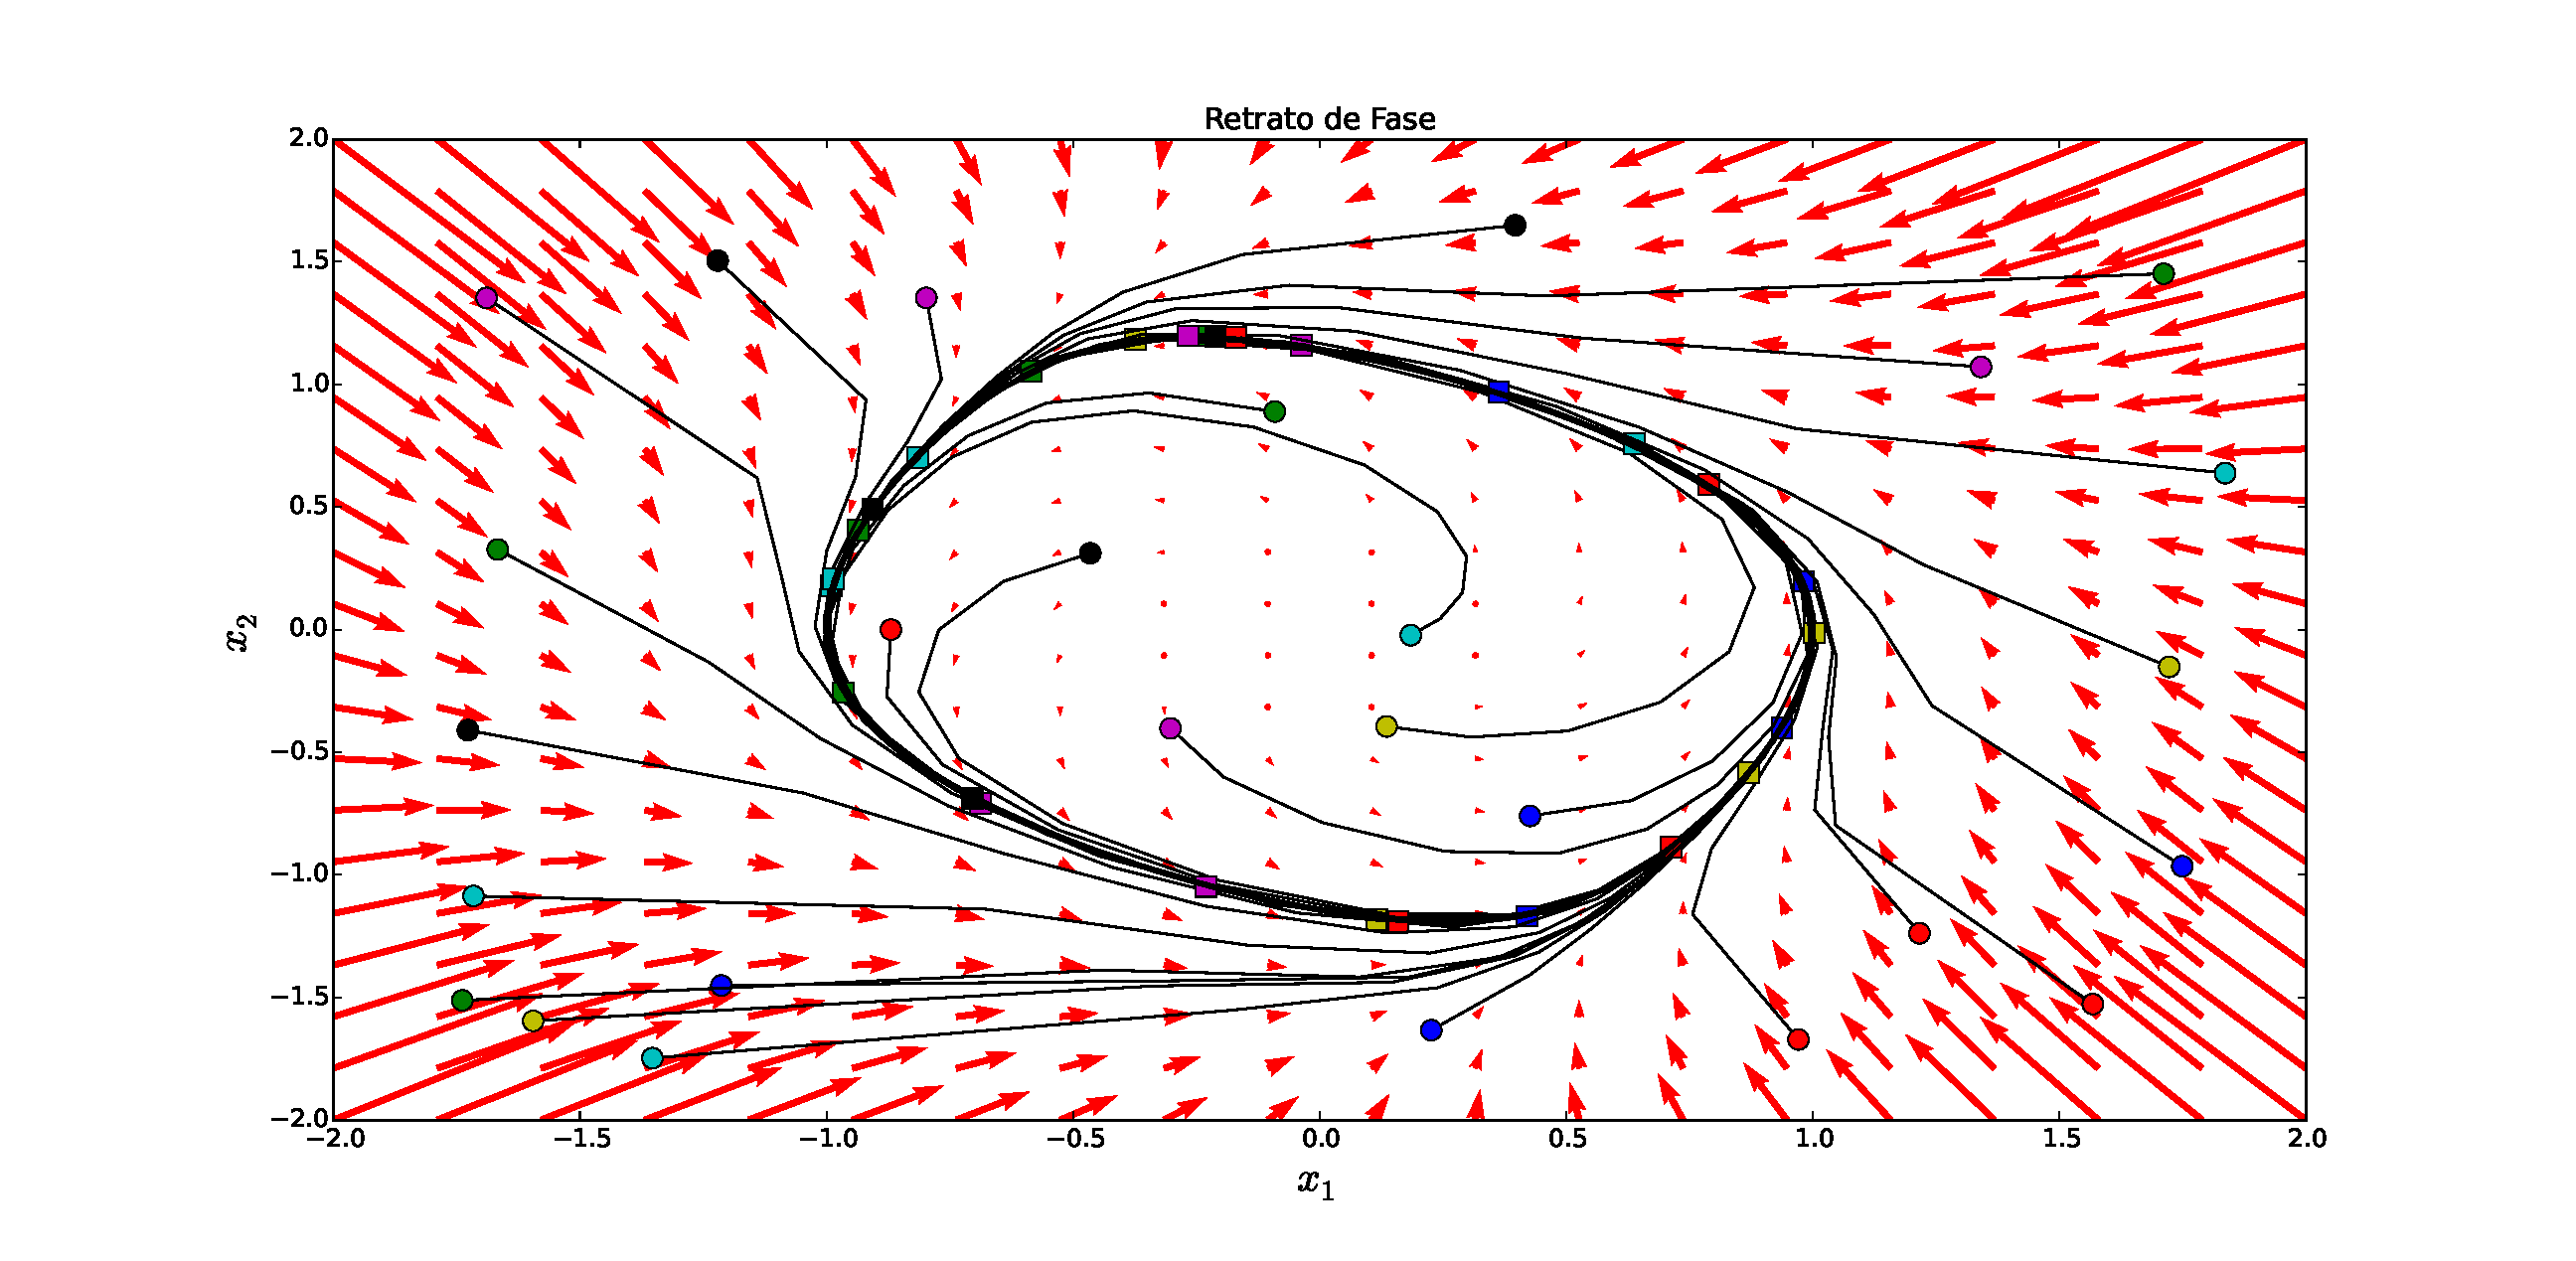
\includegraphics[width=0.97\textwidth]{phase_portrait.eps}
   \caption{Retrato de fase del sistema \eqref{eq:problema1}}\label{fig:retrato_de_fase}     
\end{figure}

%-------------------------------------------------------------------------
% Problema 2
%-------------------------------------------------------------------------
\section{Problema 2}
Dado el sistema:

\begin{equation}
     \label{eq:problema2}
      \left\{
	       \begin{array}{ll}
               \dot{x_{1}}=2x_{2}+x_{1}(x_{1}^{2}+2x_{2}^{4})\\[5pt] %truco para agregar espacio
               \dot{x_{2}}=-2x_{1}+x_{2}(x_{1}^{2}+x_{2}^{4})
	       \end{array}
	     \right.
\end{equation}
Analizar la estabilidad del punto de equilibrio.

\subsection{Resolución}

Primero la definición de estabilidad de un punto de equilibrio es la siguiente:


\begin{defi}[Estabilidad PE] 
    El punto de equilibrio (PE) $x=0$ es:
  \begin{itemize}
    \item \textit{estable}, si para cada $\epsilon > 0$ existe un $\delta = \delta(\epsilon)$ tal que:
        \begin{equation}
            \Vert x(0) \Vert < \delta \Longrightarrow \Vert x(t) \Vert < \epsilon \quad  \forall \, t \geq t_0 \label{eq:est_uni}
        \end{equation}

    \item \textit{inestable} si no es estable 
     
    \item \textit{asintóticamente estable}(AE) si es estable y $\delta$ puede elegirse tal que:
        \begin{equation}
            \Vert x(0) \Vert < \delta \Longrightarrow \lim \limits_{t \rightarrow \infty}x(t)=0
        \end{equation}
    \end{itemize}
\end{defi}

Además una de las herramientas clásicas en la teoría de estabilidad es el teorema de Lyapunov
\begin{teo}[Lyapunov]
    Sea el origen $x=0$ un PE de \eqref{eq:forma_vec} y sea $D \subset \mathbb{R}^{n}$ un dominio
    que contiene el origen. Sea $V$: $D \rightarrow \mathbb{R}$ una función continuamente diferenciable tal que:
    \begin{equation}
        V(0)=0 \quad y \quad V(x) > 0 \quad en \quad D-{0} \label{eq:def_pos}
    \end{equation}
    
    \begin{equation}
        \dot{V}(x) \leq 0 \quad en \quad D
    \end{equation}
    Entonces $x=0$ es estable. Más aún, si 
    \begin{equation}
        \dot{V}(x) < 0 \quad en \quad D
    \end{equation}
    entonces $x=0$ es Asintóticamente estable(AE)
\end{teo}

Además con un tratamiento muy parecido para la estabilidad podemos clasificar a un PE como inestable gracias al 
siguiente resultado:

\begin{teo}[Chetaev]
    Sea $x=0$ un PE de \eqref{eq:forma_vec}. Sea $V \rightarrow \mathbb{R} $ una función continuamente diferenciable
    tal que $V(0)=0$ y $V(x_{0})>0$ para algún $x_{0}$ con $\Vert x_{0} \Vert$ arbitrariamente pequeña. Definamos el 
    Conjunto $U$ como:
    \begin{equation}
        U = \left\{x \in B_{r} | V(x) > 0 \right\}
    \end{equation}
    \begin{equation}
        B_{r} = \left\{ x \in \mathbb{R}^{n}|\Vert x \Vert \leq r \right\}
    \end{equation}
    y supongamos que $\dot{V} > 0 $ en $U$. Entonces $x=0$ es inestable.
    \label{Chetaev}
\end{teo}
Además otro resultado muy poderoso conocido como \textit{metodo indirecto de Lyapunov}, el cual da condiciones 
para determinar la estabilidad del origen del sistema no lineal, a traves del estudio de la estabilidad del sistema linealizado.

\begin{teo}[Metodo indirecto de Lyapunov]
    Sea $x=0$ un PE del sistema no lineal \eqref{eq:forma_vec} donde $f:D \rightarrow \mathbb{R}^{n}$ es una función continuamente
    diferenciable y $D \subset \mathbb{R}^{n}$ es un entorno del origen. Sea:
     \begin{equation}
        A=\dfrac{\partial \mathbf{f}}{\partial \mathbf{x}}\bigg\vert_{\mathbf{x}=\mathbf{0}}=
        \begin{bmatrix}
            \dfrac{\partial f_1}{\partial x_1}& \dfrac{\partial f_1}{\partial x_2} \\ 
            \dfrac{\partial f_2}{\partial x_1}& \dfrac{\partial f_2}{\partial x_2}
        \end{bmatrix} 
        \bigg\vert_{\mathbf{x}=\mathbf{0}}
    \label{eq:jaco2}
    \end{equation}
    Entonces:
    \begin{itemize}
            \item El origen es asintoticamente estable(AE) si todos los autovalores de $A$ tienen parte real negativa
            \item El origen es inestable si uno o más autovalores de $A$ tienen parte real positiva.
    \end{itemize}
\label{lyapunov_indirecto}
\end{teo}

Primero comenzamos calculando los puntos de equilibrio del sistema \eqref{eq:problema2}

Obtenemos nuevamente que el único punto de equilibrio del sistema es: $\mathbf{x}^{*} = (0,0)$

Primero investiguemos si podemos inferir el comportamiento cualitativo del PE a traves de su linealización. Para ello calculamos 
la matriz Jacobiana del  sistema:




\begin{equation}
\dfrac{\partial \mathbf{f}}{\partial \mathbf{x}}=
\begin{bmatrix}
 \dfrac{\partial f_1}{\partial x_1}& \dfrac{\partial f_1}{\partial x_2} \\ 
\dfrac{\partial f_2}{\partial x_1}& \dfrac{\partial f_2}{\partial x_2}
\end{bmatrix} 
=
\begin{bmatrix}
  3 x_{1}^{2} + 2 x_{2}^{4} & 8 x_{1} x_{2}^{3} + 2\\
 2 x_{1} x_{2} - 2 & x_{1}^{2} + 5 x_{2}^{4}
\end{bmatrix}
\label{eq:jaco_sis2}
\end{equation}



Luego al evaluar la matriz Jacobiana en el PE obtenemos:
\begin{equation}
A_2=\dfrac{\partial \mathbf{f}}{\partial \mathbf{x}}\bigg\vert_{\mathbf{x}=\mathbf{x}_1}=
\begin{bmatrix}
0 & 2 \\
-2& 0
\end{bmatrix}
\label{eq:jaco_sis_2}
\end{equation}


Cuyos autovalores son:

\begin{equation}
    \lambda_{1}^{A_{2}}=-2j    \label{eq:raiz_1_2}
\end{equation}


\begin{equation}
    \lambda_{2}^{A_{2}}=2j \label{eq:raiz_2_2}
\end{equation}

Ya que los puntos no son hiperbólicos(son imaginarios puros) no podemos inferir el comportamiento ni la estabilidad del PE 
directamente. Por ello Sea la función $V(\mathbf{x}) = x_{1}^{2} + x_{2}^{2}$ una función definida positiva $\forall$ $\mathbf{x}$ $\in$ $\mathbb{R}^{2}$. Luego Sea:
\begin{equation}
    \dot{V}(\mathbf{x}) = \frac{\partial V}{\partial \mathbf{x}}\dot{\mathbf{x}}=\frac{\partial V}{\partial \mathbf{x}}\mathbf{f}
\end{equation}

\begin{equation}
    \dot{V}(\mathbf{x})=2x_{1}f_{1} + 2x_{2}f_{2}
\end{equation}
Lo que nos da:

\begin{equation}
     \dot{V}(\mathbf{x})=2 x_{1}^{4} + 4 x_{1}^{2} x_{2}^{4} + 2 x_{1}^{2} x_{2}^{2} + 2 x_{2}^{6}
\end{equation}

Como vemos $\dot{V}(\mathbf{x})> 0$  $\forall$ $\mathbf{x} \in \mathbb{R}^{2}$ Aplicando el teorema de Chetaev \ref{Chetaev} concluimos que el PE es \textit{inestable}.



%-------------------------------------------------------------------------
% Problema 3
%-------------------------------------------------------------------------

\section{Problema 3}

Dado el sistema:


\begin{equation}
     \label{eq:problema3}
      \left\{
	       \begin{array}{ll}
               \dot{x_{1}}=-x_{1}^{3}+u\\[5pt] %truco para agregar espacio
               \dot{x_{2}}=x_{1}
	       \end{array}
	     \right.
\end{equation}
Analizar la estabilidad del punto de equilibrio para $u=0$ y $u=-x_{2}$


Primero para el caso $u=0$ el sistema que nos queda es:

\begin{equation}
     \label{eq:problema3_2}
      \left\{
	       \begin{array}{ll}
               \dot{x_{1}}=-x_{1}^{3}\\[5pt] %truco para agregar espacio
               \dot{x_{2}}=x_{1}
	       \end{array}
	     \right.
\end{equation}

En este caso tenemos un conjunto de puntos de equilibrio que es toda la recta $x_{1}=0$. Por ello 
la linealización no nos va a ayudar a estudiar el comportamiento del sistema. Lo comprobamos con los
siguientes calculos:

\begin{equation}
\dfrac{\partial \mathbf{f}}{\partial \mathbf{x}}=
\begin{bmatrix}
 \dfrac{\partial f_1}{\partial x_1}& \dfrac{\partial f_1}{\partial x_2} \\ 
\dfrac{\partial f_2}{\partial x_1}& \dfrac{\partial f_2}{\partial x_2}
\end{bmatrix} 
=
\begin{bmatrix}
    -3x_{1}^{2} & 0\\
1 & 0 
\end{bmatrix}
\label{eq:jaco_sis3}
\end{equation}

Como esperabamos la linealización nos da cero como autovalor doble del sistema linealizado. 
Una herramienta de la que podemos hacer uso en este caso es el siguiente teorema:

\begin{teo}[LaSalle]
    Sea $\Omega \subset D$  un conjunto compacto que es invariante positivo com respecto a \eqref{eq:forma_vec}. Sea 
    $V:\, D \rightarrow \mathbb{R} $ una función continuamente diferenciable tal que $V(\mathbf{x}) \leq 0$ en $\Omega$. Sea 
    $E$ el conjunto de todos los puntos de $\Omega$ donde $V(\mathbf{x})=0$. Sea $M$ el mayor conjunto invariante en $E$. Entonces 
    toda solución que comienza en $\Omega$ tiende a $M$ cuando $t \rightarrow \infty$
\end{teo}

Sea $V(\mathbf{x})=x_{1}^{2}$(Notemos que el teorema no pide que $V(\mathbf{x})$ sea definida positiva), 
\begin{equation}
    \Omega_{c} = \left\{\mathbf{x} \in \mathbb{R}^{2}| V(\mathbf{x}) \leq c \quad x_{2} \in [b,d]\right\} 
\end{equation}

Calculamos sobre las trayectorias: 

\begin{equation}
    \dot{V}(\mathbf{x})=-6 x_{1}^{2}
\end{equation}

y sea 

\begin{equation}
    E = \left\{ x \in \Omega_{c}|x_{1}=0 \right\}
\end{equation}

El conjunto invariante que en este caso $E=M$, como se cumples las hipótesis del teorema y además como podemos elegir las constantes
$a,b,c$ para cualquier valor real, el sistema es \textit{globalmente asintoticamente estable}.


Luego para el caso en el que $u=-x_{2}$ el sistema que nos queda es:

\begin{equation}
     \label{eq:problema3_2_1}
      \left\{
	       \begin{array}{ll}
               \dot{x_{1}}=-x_{1}^{3}-x_{2}\\[5pt] %truco para agregar espacio
               \dot{x_{2}}=x_{1}
	       \end{array}
	     \right.
\end{equation}

en este caso para para el PE $\mathbf{x} = (0,0)$ 



\begin{equation}
\dfrac{\partial \mathbf{f}}{\partial \mathbf{x}}=
\begin{bmatrix}
 \dfrac{\partial f_1}{\partial x_1}& \dfrac{\partial f_1}{\partial x_2} \\ 
\dfrac{\partial f_2}{\partial x_1}& \dfrac{\partial f_2}{\partial x_2}
\end{bmatrix} 
=
\begin{bmatrix}
    -3x_{1}^{2} & -1\\
1 & 0 
\end{bmatrix}
\label{eq:jaco_sis3}
\end{equation}

cuyos autovalores son:$\lambda_{1}=i$ y $\lambda_{2}=-i$. Como no son hiperbólicos 
no podemos inferir el comportamiento del sistema linealizado. 
Sea $V(\mathbf{x})=x_{1}^{2}+x_{2}^{2}$ entonces sobre las trayectorias:

\begin{equation}
    \dot{V}(\mathbf{x}) = -2x_{1}^{4}
\end{equation}

Vemos que $\dot{V}(\mathbf{x})$ es semidefinida negativa para todo $\mathbf{x}$, entonces si $x_{1} \sim 0$ $\dot{x}_{2} \sim 0$
y entonces $x_{2} \sim 0$ y por ello $x_{1}^{3}(t) \sim 0$ entonces por el principio de invariancia el origen es globalmente asintoticamente estable.

\newpage

\begin{thebibliography}{6}
 \bibitem{Principal}{ Nonlinear Systems, third edition. Hassan K. Khalil,ISBN 0-13-067389-7 }
 \bibitem{alternativo}{Applied Nonlinear Control. Jean-Jacques E. Slotine, Weiping Li, ISBN 0-13-040890-5}
\end{thebibliography}




\end{document}
